\section{Database and Persistence Layer}
\label{sec:database_layer}

Storing the minimum necessary information is both a privacy principle and a practical simplification. Chatnalyxer's PostgreSQL schema persists only three fields per extracted task: the \texttt{Task Name}, the \texttt{ISO-8601 Deadline}, and the computed \texttt{Priority Score}. The originating \texttt{Group ID} is stored only as a one-way cryptographic hash, which means that even if the database were compromised, it would be computationally infeasible to reconstruct which chat produced a given task record (illustrated in Fig.~\ref{fig:er_diagram}). No message body, no media content, and no participant identifiers are retained after the inference window closes.

\begin{figure}[tbp]
    \centering
    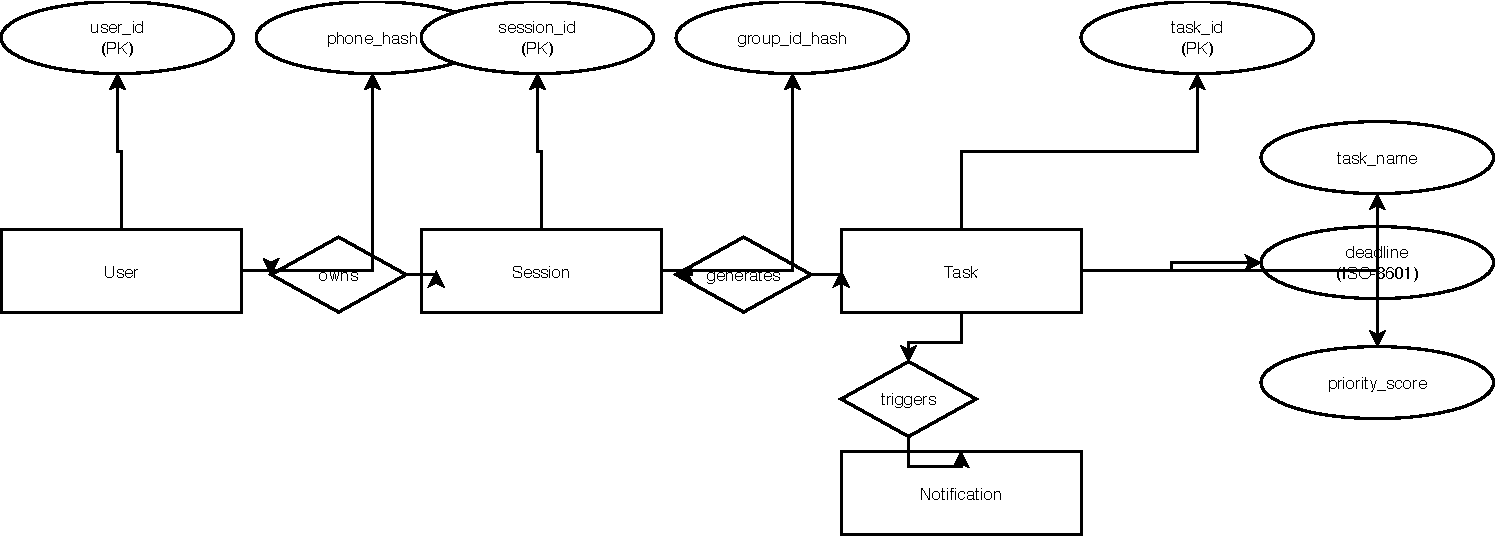
\includegraphics[width=0.95\columnwidth,keepaspectratio]{figures/Fig5_Entity_Relationship.pdf}
    \setlength{\abovecaptionskip}{4pt}
    \setlength{\belowcaptionskip}{-4pt}
    \caption{Entity-Relationship schema for the Chatnalyxer PostgreSQL cluster. Group identifiers are stored as non-reversible cryptographic hashes, preventing reconstruction of conversational history even under full database exposure.}
    \label{fig:er_diagram}
\end{figure}

This schema design was driven by a specific threat model: a background listener that retains conversational content is a high-value surveillance target. By strictly constraining full message retention at the architectural level—not merely via policy—the design mitigates a significant class of privacy risks at the data layer.
